%% Copernicus Publications Manuscript Preparation Template for LaTeX Submissions
%% ---------------------------------
%% This template should be used for copernicus.cls
%% The class file and some style files are bundled in the Copernicus Latex Package, which can be downloaded from the different journal webpages.
%% For further assistance please contact Copernicus Publications at: production@copernicus.org
%% https://publications.copernicus.org/for_authors/manuscript_preparation.html


%% Please use the following documentclass and journal abbreviations for discussion papers and final revised papers.

%% 2-column papers and discussion papers
\documentclass[gmd, manuscript]{copernicus}

\usepackage{graphicx}
\usepackage{natbib}


\usepackage{tikz}
\tikzset{
    state/.style={
           rectangle,
           rounded corners,
           draw=black, ultra thick,
           minimum height=2em,
           inner sep=2pt,
           text centered,
           text width=40ex
           },
}

%% Journal abbreviations (please use the same for discussion papers and final revised papers) 
% Advances in Geosciences (adgeo)
% Advances in Radio Science (ars)
% Advances in Science and Research (asr)
% Advances in Statistical Climatology, Meteorology and Oceanography (ascmo)
% Annales Geophysicae (angeo)
% Archives Animal Breeding (aab)
% ASTRA Proceedings (ap)
% Atmospheric Chemistry and Physics (acp)
% Atmospheric Measurement Techniques (amt)
% Biogeosciences (bg)
% Climate of the Past (cp)
% DEUQUA Special Publications (deuquasp)
% Drinking Water Engineering and Science (dwes)
% Earth Surface Dynamics (esurf)
% Earth System Dynamics (esd)
% Earth System Science Data (essd)
% E&G Quaternary Science Journal (egqsj)
% Fossil Record (fr)
% Geographica Helvetica (gh)
% Geoscientific Instrumentation, Methods and Data Systems (gi)
% Geoscientific Model Development (gmd)
% History of Geo- and Space Sciences (hgss)
% Hydrology and Earth System Sciences (hess)
% Journal of Micropalaeontology (jm)
% Journal of Sensors and Sensor Systems (jsss)
% Mechanical Sciences (ms)
% Natural Hazards and Earth System Sciences (nhess)
% Nonlinear Processes in Geophysics (npg)
% Ocean Science (os)
% Primate Biology (pb)
% Proceedings of the International Association of Hydrological Sciences (piahs)
% Scientific Drilling (sd)
% SOIL (soil)
% Solid Earth (se)
% The Cryosphere (tc)
% Web Ecology (we)
% Wind Energy Science (wes)


%% \usepackage commands included in the copernicus.cls:
%\usepackage[german, english]{babel}
%\usepackage{tabularx}
%\usepackage{cancel}
%\usepackage{multirow} 
%\usepackage{supertabular}
%\usepackage{algorithmic}
%\usepackage{algorithm}
%\usepackage{amsthm}
%\usepackage{float}
%\usepackage{subfig}
%\usepackage{rotating}

%% New commands for paper drafting process:
\newcommand{\CONTRIBUTORS}[1]{\textcolor{green}{\textsf{\textsl{CONTRIBUTORS: #1}}}}
\newcommand{\TODO}[1]{\textcolor{blue}{\textsf{\textbf{TODO: #1}}}}

\begin{document}

\title{ACCESS-OM2: A Global Ocean-Sea Ice Model at Three Resolutions}


% \Author[affil]{given_name}{surname}

\Author[1]{Andrew E.}{Kiss}
\Author[1]{Andrew McC.}{Hogg}
\Author[2]{Nicholas}{Hannah}
\Author[3]{Gary}{Brassington}
\Author[6]{Christopher}{Chapman}
\Author[13]{Fabio}{Dias}
\Author[13,6]{Peter}{Dobrohotoff}
\Author[13]{Catia}{Domingues}
\Author[5]{Matthew H.}{England}
\Author[6]{Russell}{Fiedler}
\Author[7]{Stephen M.}{Griffies}
\Author[1]{Aidan}{Heerdegen}
\Author[13,8]{Petra}{Heil}
\Author[5,12]{Ryan M.}{Holmes}
\Author[6]{Simon J.}{Marsland}
\Author[1]{Adele K.}{Morrison}
\Author[9]{James}{Munroe}
\Author[6]{Peter}{Oke}
\Author[4]{Andreas}{Klocker}
\Author[13]{Maxim}{Nikurashin}
\Author[6]{Oc\'eane}{Richet}
\Author[13]{Abhishek}{Savita}
\Author[5]{Paul}{Spence}
\Author[1]{Kial D.}{Stewart}
\Author[10]{Marshall}{Ward}
\Author[11]{Fanghua}{Wu}
\affil[1]{Research School of Earth Sciences and ARC Centre of Excellence for Climate Extremes, Australian National University}
\affil[2]{Double Precision}
\affil[3]{BoM}
\affil[4]{Antarctic Climate and Ecosystems Cooperative Research Centre, University of Tasmania, Hobart, Australia}
\affil[5]{Climate Change Research Centre and ARC Centre of Excellence for Climate Extremes, University of New South Wales}
\affil[6]{CSIRO}
\affil[7]{NOAA/GFDL and Princeton University Atmospheric \& Oceanic Sciences Program}
\affil[8]{AAD}
\affil[9]{Memorial}
\affil[10]{NCI}
\affil[11]{Beijing Climate Centre}
\affil[12]{School of Mathematics and Statistics, University of New South Wales}
\affil[13]{UTas}

%% The [] brackets identify the author with the corresponding affiliation. 1, 2, 3, etc. should be inserted.



\runningtitle{ACCESS-OM2}

\runningauthor{Kiss et al.}

\correspondence{Andrew E. Kiss (Andrew.Kiss@anu.edu.au)}



\received{}
\pubdiscuss{} %% only important for two-stage journals
\revised{}
\accepted{}
\published{}

%% These dates will be inserted by Copernicus Publications during the typesetting process.

\firstpage{1}

\maketitle

\CONTRIBUTORS{Have a look at the technical report for some useful information and references:\\
\url{https://github.com/OceansAus/ACCESS-OM2-1-025-010deg-report:w
}}

\begin{abstract}
We introduce a new version of the ocean-sea ice implementation of the Australian Community Climate and Earth System Simulator, ACCESS-OM2.
The model has been developed with the aim of being aligned as closely as possible with the fully coupled (atmosphere-land-ocean-sea ice) ACCESS-CM2.
In addition, the model is available at three different resolutions: a coarse resolution (nominally 1$^\circ$), an eddy-permitting resolution (nominally 0.25$^\circ$) and an eddy-rich resolution (0.1$^\circ$ with 75 vertical levels).
The different resolutions have been developed simultaneously, both to allow testing at low resolutions and to permit comparison across resolutions.
Here, the model is introduced and the individual components are documented. 
The model performance is evaluated across the three different resolutions, highlighting the relative advantages and disadvantages of running ocean-sea ice models at higher resolution.
\end{abstract}


\copyrightstatement{TEXT}


\introduction  %% \introduction[modified heading if necessary]

Ocean-sea ice models have extensive applications.
They form the oceanic component of coupled climate and Earth system models that are used for projecting future climate, and can incorporate biogeochemical and ecosystem dynamics which extend the realm of application.
They are also needed for forecasting on shorter timescales -- both forecasting in the ocean and for seasonal prediction of the ocean/sea ice/atmosphere state.
As a research tool, ocean-sea ice models can be used to quantitatively test, or experiment with, the dynamics of the climate system; such process studies have been invaluable in forming a broad understanding of the drivers of climate change and variability.

Modelling studies face the universal challenge of the compromise between resolving critical processes and computational expense.
For example, the standard resolution for the ocean component of coupled climate models is 1$^\circ$, with indications that some models being prepared for the next Coupled Model Intercomparison Project (CMIP6) will use 0.25$^\circ$ horizontal resolution.
However, 1$^\circ$ models do not resolve the ocean mesoscale, meaning that they miss key processes that can influence the climate. 
Higher resolution models have an improved climate state with better estimates of vertical heat transport \citep{Griffies2015}, enhancement of boundary currents \citep{Hewitt2016}, better resolution of ocean straits and improved Southern Ocean state \citep{Bishop2016}.
On the other hand, these high resolution simulations consume huge computational resources, which limits the length of runs and the ability to run multiple tests to optimise parameters.
Thus, while higher resolution models are becoming computationally feasible, the additional resolution does not necessarily result in improved simulations.

One of the complexities in characterising model performance as a function of resolution is the influence of model biases governing the model state.
It is well known that different models subjected to the same forcing produce widely varying mean states \citep[e.g.][]{Danabasoglu2014}.
It follows that the effects of model resolution require a clean hierarchy; a model suite in which variations in resolution are available with homogeneous code, forcing and, as far as possible, parameter choices.
This is a technique successfully employed by the DRAKKAR consortium \citep{Barnier2006} as well as climate model developers \citep[e.g.][]{Hewitt2016}.

In this manuscript we outline the development of the latest version of the ocean-sea ice component of the Australian Community Climate and Earth System Simulation, known as ACCESS-OM2.
This model is being developed to serve the twin aims of underpinning climate model development and ocean state forecasting; it therefore includes parallel development of low, medium and high resolution options.
The model is also designed to be used for process model studies. 
In this manuscript we aim to document the model formulation (\S 2) and the computational performance of the model at each resolution (\S3).
We also undertake a preliminary evaluation of the global model state, included selected regional analyses and the model representation of sea ice (\S4).

\section{Model Formulation}
\CONTRIBUTORS{This section is currently being drafted as part of the ACCESS-OM2 technical report by Andrew Kiss. Once complete, a cut-down version of the technical report will be included here.}

Model configurations at three horizontal resolutions have been developed, named ACCESS-OM2 (nominally 1$^\circ$ horizontal resolution), ACCESS-OM2-025 (nominally 0.25$^\circ$) and ACCESS-OM2-01 (nominally 0.1$^\circ$).
The suite of three resolutions is also collectively referred to as ACCESS-OM2.
Configurations (e.g.\ run parameters and forcing) are as consistent as possible across the three resolutions to facilitate studies of resolution dependence and sub-gridscale parameterisations. 
The coarser models served as testbeds for developing correct configurations at higher resolutions, and are suitable for long experiments covering climatological timescales of hundreds of years, but are not eddy-resolving.
%They are intended for incorporation into future versions of the ACCESS-CM global coupled climate model.
In contrast, the ACCESS-OM2-01 configuration resolves the first baroclinic deformation radius away from shelves and equatorward of about 50$^\circ$ \citep{Hallberg2013a}, and therefore resolves the mesoscale in most of the world ocean. 
%It is suitable for runs of several decades and is intended to form the basis of the next generation of the Bluelink operational ocean forecasting system.

ACCESS-OM2 consists of two-way coupled ocean and sea ice models driven by a prescribed atmosphere (see Figure~\ref{F:coupling}).
The ocean model component is the Modular Ocean Model (MOM) version 5.1 from the Geophysical Fluid Dynamics Laboratory (\url{https://mom-ocean.github.io}), and the sea ice component (\url{https://github.com/OceansAus/cice5/}) is a fork from the Los Alamos sea ice model (CICE) version 5.1.2 from Los Alamos National Laboratories (\url{https://github.com/CICE-Consortium/CICE-svn-trunk/tree/cice-5.1.2}).
These components are forced by prescribed atmospheric conditions taken from the 55-year Japanese Reanalysis for driving oceans \citep[JRA55-do,][]{TsujinoETAL2018a} via YATM (\url{https://github.com/OceansAus/libaccessom2/}).
The model components are coupled via Ocean Atmosphere Sea Ice Soil (OASIS3-MCT) version 2.0 from CERFACS and CNRS, France (\url{https://portal.enes.org/oasis}).
%The exact source code and inputs used for the experiments discussed here are listed in Table~\ref{T:configs}.
The ACCESS-OM2 model source code is hosted at \url{https://github.com/OceansAus/access-om2}.
\TODO{push control directories to GitHub}
\TODO{v1.0 annotated tag for all model components and control dirs}
The following subsections provide further details on these model components.

\begin{figure}
    \begin{center}
    {\footnotesize
        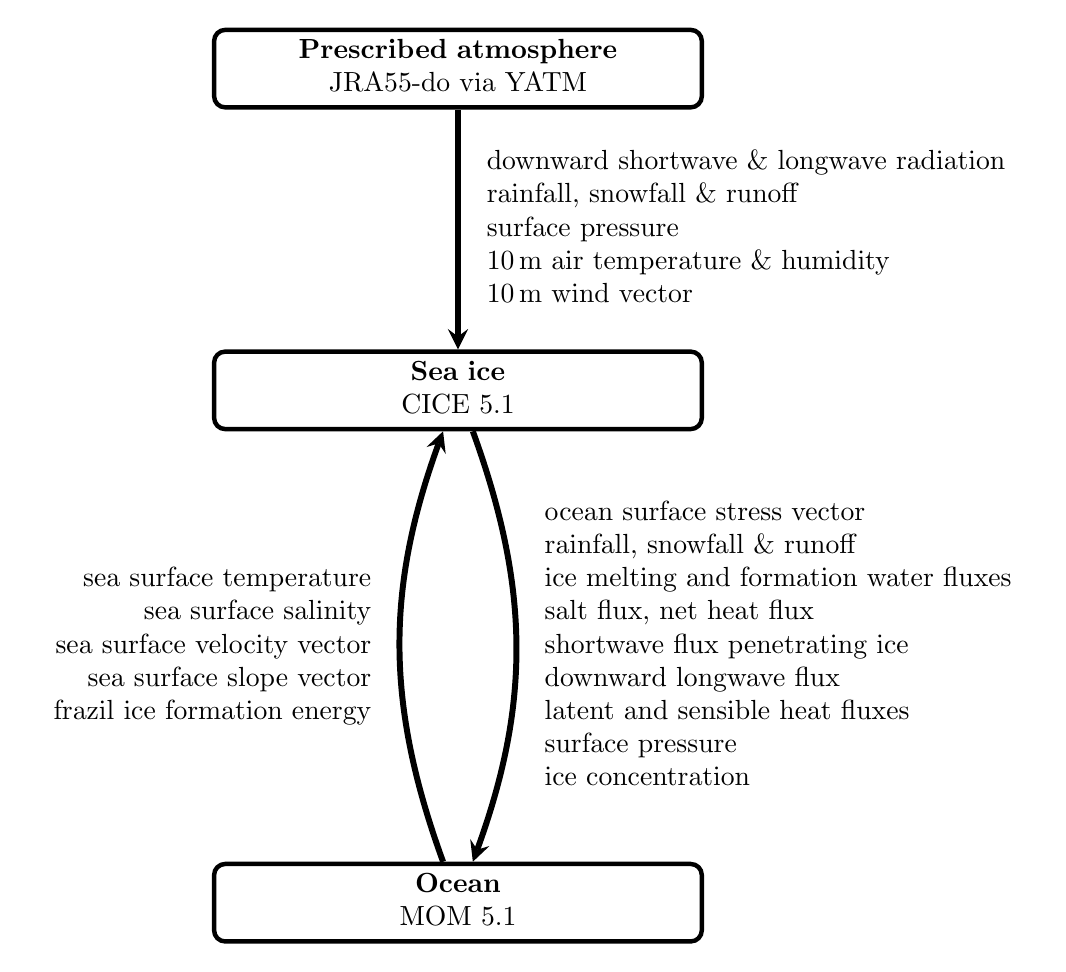
\begin{tikzpicture}[->,>=stealth,thick]
            
%             \node[state, text width=30ex] (ATM) 
             \node[state] (ATM) 
             {\begin{tabular}{c}
              \textbf{Prescribed atmosphere}\\
              JRA55-do via YATM
              \end{tabular}};
              
             \node[state, 
%              text width=30ex, 	% max text width
              below of=ATM,
              node distance=27ex,
              anchor=center] (ICE)
             {%
             \begin{tabular}{c}
              \textbf{Sea ice}\\
              CICE 5.1
             \end{tabular}
             };
             
             \node[state,
%               text width=30ex,
             below of=ICE,
              node distance=43ex,
              anchor=center
              ] (OCEAN) 
             {%
             \begin{tabular}{c}
              \textbf{Ocean}\\
              MOM 5.1
             \end{tabular}
             };
            
             \path 
             (ATM) 	edge[line width=.5ex] node[anchor=south,right]
            {
            \begin{tabular}{l}
                downward shortwave \& longwave radiation\\
                rainfall, snowfall \& runoff\\
                surface pressure\\
                10\,m air temperature \& humidity\\ % NB: namcouple comment is out of date - TsujinoETAL2018a state this is 10m (rather than 2m)
                10\,m wind vector
            \end{tabular}
            }
                (ICE)
             (ICE)  	edge[bend left=20, line width=.5ex]                  node[anchor=left,right]
             {
            \begin{tabular}{l}
                ocean surface stress vector\\
                rainfall, snowfall \& runoff\\
                ice melting and formation water fluxes\\
                salt flux, net heat flux\\
                shortwave flux penetrating ice\\
                downward longwave flux\\
                latent and sensible heat fluxes\\
                surface pressure\\
                ice concentration
            \end{tabular}
            }
            (OCEAN)            
            (OCEAN)  	edge[bend left=20, line width=.5ex]  node[anchor=left,left]
             {
            \begin{tabular}{r}
                sea surface temperature\\
                sea surface salinity\\
                sea surface velocity vector\\
                sea surface slope vector\\
                frazil ice formation energy
            \end{tabular}
            }
            (ICE)
            ;
        
        \end{tikzpicture}
        }
    \end{center}
    \caption[Coupling between model components.]{
    Coupling between model components by OASIS3-MCT.
    Notice that MOM receives atmospheric forcing via CICE rather than directly from YATM (CICE has the same global domain as MOM).
}
    \label{F:coupling}
\end{figure}

\subsection{MOM ocean model}
The primary MOM 5 reference is \citet{Griffies2012a}.
\subsubsection{Vertical grid}
We use a hydrostatic and Boussinesq (volume-conserving) ocean formulation on an Arakawa B-grid, with a free surface and $z^*$ vertical coordinate.
\subsubsection{Horizontal grid}
\subsubsection{Topography}

\subsection{CICE sea ice model}
\subsection{Forcing}
\subsection{Coupling}

\section{Computational Performance}
\CONTRIBUTORS{Andy Hogg \& Marshall Ward.}

The computational performance of a coupled model depends upon the individual performance of each of the component models, as well as the load balancing between each component.
The computational load for ACCESS-OM2 is dominated by MOM5, \TODO{check} with a modest contribution from CICE5 and negligible load from the coupling and file-based atmospheric input.
Therefore, we first investigate in detail MOM5 scalability across a wide variety of core counts.
Despite playing a smaller computational role, the performance of CICE5 plays limits the scalability of the coupled model, and performance is also variable.
Finally, the performance of the fully coupled model is inferred from the independent performance of CICE5 and MOM5, leading to recommended standard configurations.
All simulations were performed on Raijin, the peak machine at Australia's National Computation Infrastructure.
\TODO{provide a few details on raijin hardware - eg is it communication, memory or io bound for this application?}

\subsection{MOM5 Scalability}
\TODO{Marshall - please check these details! }

We conduct a series of tests into the scalability of MOM5 at each of the three model resolutions tested here.
In each test we record the main loop runtime per baroclinic timestep for 3 short simulations over a prescribed core count, and repeat this test for different numbers of core counts.
The length of each simulation in model time is set to ensure a runtime of approximately 3 minutes, and varies from 2 months at the lowest resolution to 1 day at the highest resolution.
We report the runtime per model timestep (Fig. \ref{fig:scaling_ocn}a) and the total CPU time (Fig. \ref{fig:scaling_ocn}b) for each configuration.
Each point denotes the average runtime over all MPI ranks for each run.
Note that the numbers provided here do not include startup time, which can add considerable cost especially at high core counts.

\begin{figure}[t]
\includegraphics[width=12cm]{scaling_ocn.png}
\caption{Scaling performance for MOM5 global model simulations showing (a) walltime, and (b) CPU time per ocean baroclinic timestep for a short simulation at each model resolution. \label{fig:scaling_ocn}}
\end{figure}

These tests demonstrate the highly efficient scalability of MOM5. 
For the standard (1$^\circ$ resolution) ACCESS-OM2 configuration, the model scales well to core counts of 400, and only begins to degrade at 800 cores.
At 400 cores, one model year takes just 10 minutes (equivalent to a theoretical maximum of 144 model years per day) which far exceeds the required performance for such a model.
At higher resolution, MOM5 is slower, but still scales outstandingly well -- up to 4000 cores for ACCESS-OM2-025 and 16,000 cores for ACCESS-OM2-01.
In the latter case, MOM5 alone could simulate a theoretical maximum of almost 5 years per day at 0.1$^\circ$ resolution, although startup and model I/O would reduce the speed in any practical case.

These scaling tests highlight the efficiency of MOM5 at high core counts, giving us flexibility to choose different MOM5 core counts for different configurations.
However, the behaviour of the coupled model is also dependent on CICE5 performance, as outlined below.

\subsection{CICE Scalability}
\CONTRIBUTORS{Andy Hogg \& Marshall Ward.}
\TODO{This section will show graphs of CICE5  scalability (?at each of the 3 resolutions?). It will show that CICE can scale quite well,  but that load balancing can be an issue. It might also be nice to show seasonal variability in CICE, the dependence of the amount of work on latitude (model state?) and how maxblocks results in an improvement in performance for large core counts.}

\subsection{Coupled Model Performance}
\CONTRIBUTORS{Andy Hogg \& Marshall Ward.}
\TODO{This section will outline the complexities of putting together the above scaling numbers into a fully coupled model. The point is that the coupling overhead is small, but that load balancing remains a big issue, especially if timesteps vary, the model state changes, etc...}

The standard configurations, core counts and computational costs of differing model resolutions is shown in table \ref{tab:perf} \ldots



\begin{table}
\caption{A preliminary outline of model grid, size and performance. These numbers are approximate and need to be confirmed. \label{tab:perf}}
\begin{tabular}{lcccccccc}
\hline
\textbf{Model} & Lateral  & Model & Vertical  & minimum & Ocean & Cores & Walltime & CPU\\
& Spacing & Domain & Levels &  $\delta z$ (m) & Timestep (s)&  & (years/day) & (hours/year)\\
\hline
ACCESS-OM2 & 1$^\circ$ & $360 \times 300$ & 50 & 2.3~m & 5400 & 252 & 60 & 160\\
ACCESS-OM2-025 & 0.25$^\circ$ & $ 1440 \times 1080 $ & 50 & 2.3~m & 1800 & 1824 & 16 & 2,800\\
ACCESS-OM2-01 & 0.1$^\circ$ & $3600 \times 2700$ & 75 & 1.2~m & 600 & 5744 & 2.2  & 63,000\\
\hline
\end{tabular}
\end{table}
\section{Model evaluation}
We now proceed to outline results from initial simulations with ACCESS-OM2 using simulations with each of the three standard horizontal resolutions, nominally: 
\begin{itemize}
\item 1$^\circ$ with 50 vertical levels (referred to as the default version of ACCESS-OM2); 
\item 0.25$^\circ$ with 50 vertical levels (ACCESS-OM2-025); and
\item 0.1$^\circ$ with 75 vertical levels based on \citet{Stewart2017a} (ACCESS-OM2-01).
\end{itemize}
Each of the three simulations is forced by the interannual JRA55-do forcing dataset  \citep{TsujinoETAL2018a}, which  currently covers 60 years from 1958 until the end of 2017.
The  lower resolution simulations (both ACCESS-OM2 and ACCESS-OM2-025) continuously run through five iterations of this dataset, giving a 300-year simulation.
These simulations are shown by the orange and blue lines in figure \ref{fig:timeseries}, where dates have been aligned so that the last cycle of forcing matches the calendar dates of the forcing dataset (giving a nominal start year of 1718).
The main period of model evaluation will be the final interannual forcing cycle, years 1958--2017 inclusive.

\begin{figure}[t]
\includegraphics[width=12cm]{GlobalTimeseries.pdf}
\caption{Timeseries of the global average of (a) temperature; (b) surface salinity; (c) sea level and (d) kinetic energy for each of the simulations. 
Output is shown for the full interannually forced model simulations, including 5 IAF cycles for ACCESS-OM2 and ACCESS-OM2025.
Time has been offset to ensure that the final cycle has a date that is consistent with the forcing date, allowing the short, 33 year, ACCESS-OM2-01 simulation to be plotted on the same time axis.\label{fig:timeseries}}
\end{figure}

The highest resolution simulation, using ACCESS-OM2-01, is $O(1000)$ times more computationally intensive than ACCESS-OM2, and $O(30)$ times more computationally intensive than ACCESS-OM2-025.
A full simulation with five internannual forcing cycles of ACCESS-OM2-01 is not possible with current computing resources, and hence we use an alternative spinup strategy. 
In this case we select a Repeat Year Forcing (RYF) spinup strategy (Stewart et al., Paper in Prep.), in which the time period May 1984 to April 1985 is repeated continuously.
This spinup has been run for 40 years, after which time we conduct an interannually forced simulation from 1985 through to 2017. 
It is this interannual simulation period which is used for the model evaluation shown here, as indicated by the green line in figure \ref{fig:timeseries}.
It is important to note that this simulation is less well equilibrated than the lower resolution simulations, and so care must be taken in interpreting the influence of model drift on the different cases.

The timeseries of globally averaged quantities shown in figure \ref{fig:timeseries} indicate that there is a drift due to  heat uptake in ACCESS-OM2-025, while ACCESS-OM2-01 drifts cold relative to the initial state (Fig. \ref{fig:timeseries}a).
The high resolution model also drifts towards surface freshening, which is partly offset by the surface salinity restoring that is incorporated into the model (Fig. \ref{fig:timeseries}b).
The global sea surface height variation is dominated by the interannual forcing cycle, and is independent of resolution (Fig. \ref{fig:timeseries}c). 
As expected, the kinetic energy of the simulations is a strong function of resolution, with higher resolution models containing more turbulent processes (Fig. \ref{fig:timeseries}d).
Each of these aspects of the simulations is investigated in greater depth by the following analysis, where we first focus on global circulation metrics, then look to better characterise important regional ocean circulation differences and finally investigate the representation of sea ice.

\subsection{Global circulation}

\subsubsection{Horizontal circulation}
One of the most commonly used integrated metrics for ocean model circulation is the transport of the Antarctic Circumpolar Current (ACC) through Drake Passage.
Figure \ref{fig:drake} shows the Drake Passage transport for the final forcing cycle for each of the three simulations being compared.
There is a clear distinction between the ACCESS-OM2-025 transport and the two other simulations.
In the former case, the larger ACC transport is close to the observational estimate of 173 Sv \citep[black dashed line; ][]{Donohue2016}, with significant decadal variability. 
The other two cases have significantly lower transport, and are more stable. 
The  Drake Passage transport in ACCESS-OM2-025 is likely controlled by the stronger abyssal circulation induced by Antarctic polynyas (shown in more detail below) which is absent in the  lower and higher resolution cases.
The low ACC transport in this model is characteristic of this class of ocean-sea ice models \citep[e.g.][]{Farneti2015}.

\begin{figure}[t]
\includegraphics[width=8.3cm]{DP_transport.pdf}
\caption{Transport through Drake Passage as a function of time for each of the 3 model simulations. The black dashed line shows the observational estimates of Donohue et al. (2016). \label{fig:drake}}
\end{figure}

To evaluate the capacity of the different model configurations to represent the mean state of the broad-scale horizontal ocean circulation, the simulated mean dynamic topography (MDT) averaged over the final 25 years of each experiment (corresponding to the years 1993--2017) is compared with the CNES-CLS13 observational product distributed by AVISO, which combines data from satellites, surface drifters and in-situ measurements to reconstruct a time mean, global MDT field for the period between 1993 and 2012. 
The reconstruction procedure is described in \citet{Rio2011}. 
The comparisons between the simulated and observed MDTs are shown in Fig. \ref{fig:mdt}, indicating broad-scale agreement in this metric.
There is a noticeable improvement in western boundary current structure in the higher resolution models, and a deeper MDT minimum in the ACCESS-OM2-025 case, consistent with the enhanced Drake Passage transport shown in Fig. \ref{fig:drake} (again, we hypothesise that lower MDT is caused by spurious polynya activity creating more dense water in this region).
\TODO{comment on apparent disagreement in Arctic?}

\begin{figure}[t]
\includegraphics[width=\hsize]{mean_dynamic_topography.png}
\caption{Mean Dynamic Topography. (a) ACCESS-OM2; (b) ACCESS-OM2-025; (c) ACCESS-OM2-01 and (d) Observations from the CNES-CLS13 product
\label{fig:mdt}}
\end{figure}

We also evaluate the capacity of the different model configurations to represent the spatial patterns of sea-level variability, as this provides a reliable proxy surface mesoscale activity. 
To do this, we compute the standard deviation of the sea-level anomaly (SLA) for each configuration, once again computed using the final 25 years of model output, at each model grid point, to produce global maps of SLA deviation. 
The simulated SLA standard deviation is then compared with the objectively interpolated, multi-mission satellite derived, SLA product (AVISO Ssalto/Duacs) distributed by Copernicus Marine and Environment Monitoring Systems. 
Statistics are calculated for the years 1993--2017 and long-term linear trends are removed. 
We use the gridded observational product for convenience in comparing global maps of SLA variability. 
However, we note that the optimal interpolation procedure used to produce the gridded product from satellite ground tracks tends to smooth the underlying fields and hence may underestimate the SLA variance by as much as 50\% in certain regions \citep{Chambers2018}. 
As such, the true SLA variability may be higher than is indicated here. 
The maps of SLA standard deviation are plotted in Fig. \ref{fig:SL-RMS}.   

Elevated SLA variability typically occurs in regions rich in energetic mesoscale eddies. 
For example, the altimetric product (Fig. \ref{fig:SL-RMS}(d)) shows elevated SLA variability in western boundary currents and their jet extensions, as well as in the Southern Ocean, which are regions where mesoscale dynamics are most active. 
Both the ACCESS-OM2-01 and ACCESS-OM-025 simulations appear to capture this spatial pattern of SLA well, with both boundary currents and the Southern Ocean playing host to regions of enhanced SLA standard deviation. 
However, the ACCESS-OM-025 configuration is unable to capture the magnitude of the observed variability, with values a factor of two or more below those of the observational product. 
In contrast, the ACCESS-OM-01 configuration accurately captures both the spatial patterns of SLA variability and their magnitudes, with the highest values being found south of the African continent in the Agulhas retroflection region, and the Gulf Stream and Kuroshio currents. 
We note here that the coarse-resolution ACCESS-OM2 configuration is unable to capture the observed SLA variability. 


\begin{figure}[t]
\includegraphics[width=\hsize]{sea_level_anomaly_rms.png}
\caption{Standard deviation of Sea Level Anomaly. (a)~ACCESS-OM2; (b)~ACCESS-OM2-025; (c)~ACCESS-OM2-01 and (d)~Observations from gridded AVISO altimetry.  
\TODO{change colourbar caption to standard deviation}
\label{fig:SL-RMS}}
\end{figure}



\subsubsection{Overturning circulation}
Figure \ref{fig:overturning} shows the overturning circulation, computed on $\sigma_2$ surfaces, averaged over the last 25 years of simulation (1993-2017) for each of the three cases.
In this figure, the positive cell which has a maximum near potential density 1036.5 kg m$^{-3}$ is the interhemispheric upper overturning cell which is dominated by the Atlantic component.
This Atlantic Meridional Overturning Circulation (AMOC) involves sinking of dense water in the North Atlantic, which re-emerges at the surface in the Southern Ocean \citep{MarshallSpeer2012a}. 
There are clear differences between the three resolutions in their ability to represent the AMOC cell, which has an estimated transport from 2004 to 2012 of 17.2\,Sv at $26^\circ$N \citep{McCarthy:2015}.
In ACCESS-OM2, the AMOC is weak, with a maximum value \TODO{specify latitude - it's about 18Sv at 50S} of around 10 Sv, but it retains a strong interhemispheric character. 
In ACCESS-OM2-025 the AMOC is much weaker in the northern hemisphere, while in ACCESS-OM2-01 the AMOC remains relatively strong.
A timeseries of the AMOC, measured at 26$^\circ$N and constrained to the Atlantic basin only, clearly shows these differences (Figure \ref{fig:overturning_timeseries}a), but also shows a decline over the duration of the ACCESS-OM2-01 case.
Longer simulations are required before we can establish the equilibrium AMOC for this model.

\begin{figure}[t]
\includegraphics[width=\hsize]{mean_overturning.png}
\caption{Time-mean zonally-integrated overturning circulation computed on $\sigma_2$ density surfaces for (a) ACCESS-OM2; (b) ACCESS-OM2-025 and (c) ACCESS-OM2-01 simulations. Overturning is computed on density surfaces, integrated zonally around the globe and averaged over the last 25 years of simulation (1993--2017). \label{fig:overturning}}
\end{figure}

The other circulation cell of interest in Figure \ref{fig:overturning} is the abyssal overturning cell (the negative cell centred at 1037 kg/m$^{-3}$), which occupies a small part of density space but comprises a significant fraction of global water volume.
Here, both ACCESS-OM2-025 and ACCESS-OM2-01 have a strong overturning cell \citep[10--15\,Sv at $40^\circ$S, see figure \ref{fig:overturning_timeseries}b; compared with poorly constrained observational estimates of 20--50,Sv;][]{Sloyan2001,Lumpkin2007,Talley2013}.
\TODO{rephrase? - 025 looks closer to 1deg than 0.1deg in timeseries and streamfunction}
However, we show below that the ACCESS-OM2-025 result occurs due to the dominance of unrealistic polynya activity in the Ross Sea, while in ACCESS-OM2-01 the abyssal cell is driven by the more realistic process of water mass transformation on the Antarctic continental shelf.
The result is the ACCESS-OM2-025 abyssal cell has large variations in strength, while the ACCESS-OM2-01 case is closer to a steady state.
On the other hand, the ACCESS-OM2 case shows some water mass transformation due to open ocean convection, but this dense water is poorly connected with the rest of the global ocean, leading to a weak ($\sim$5 Sv) \TODO{change to 8Sv?} overturning transport at 40$^\circ$S.
These biases in water mass transformation are common in coarse resolution ocean and climate models (Heuze et al)\TODO{cite}, indicating the potential of ACCESS-OM2-01 to be used for studies into the abyssal cell sensitivity to changes in climate.

\begin{figure}[t]
\includegraphics[width=12cm]{overturning_timeseries.pdf}
\caption{
\TODO{replot with groupby().mean() instead of .resample} 
(a) Upper overturning cell (AMOC) magnitude as a function of time, defined as the maximum value of the global overturning streamfunction computed on density surfaces, measured at 26$^\circ$N, integrated between 103$^\circ$W and 5$^\circ$W and for potential density classes that exceed 1035.5 kg\,m$^{-3}$. Observational estimate from \citet{McCarthy:2015} \TODO{plot this}. (b) Abyssal cell overturning magnitude as a function of time, defined as the minimum value of the global overturning streamfunction computed on density surfaces, measured at 40$^\circ$S, integrated zonally around the globe and for potential density classes exceeding 1036 kg\,m$^{-3}$. \label{fig:overturning_timeseries}}
\end{figure}


\subsubsection{Heat uptake}
\TODO{Fabio and team writing this section:} 

Figure \ref{fig:hovmoller} shows \ldots

\subsubsection{Temperature bias}
Figures \ref{fig:sstbias} and \ref{fig:zonaltemp} show...

\begin{figure}[t]
\includegraphics[width=16cm]{tz_hovmoller.png}
\caption{Uptake of heat, relative to WOA13, over last IAF cycle. \TODO{(01 case still to be computed.)} \label{fig:hovmoller}}
\end{figure}

\begin{figure}[t]
\includegraphics[width=12cm]{global_sst_bias.png}
\caption{Global SST bias from WOA13 \TODO{Add WOA data as 4th panel}\label{fig:sstbias}}
\end{figure}

\begin{figure}[t]
 \includegraphics[width=12cm]{zonal_temp_bias.png}
 \caption{Zonally averaged temperature bias relative to WOA13. \TODO{Add WOA data as 4th panel} \label{fig:zonaltemp}}
\end{figure}

\subsubsection{Heat transport} 

\begin{figure}[t]
\includegraphics[width=8cm]{meridional_heat_transport_withadv_withobs.pdf}
\caption{Meridional heat transport (PW) calculated by integrating the surface heat flux in latitude (solid lines) and from the resolved temperature advection (dashed lines).
  Observed estimates from \citet{Trenberth2001} inferred from both NCEP and ECMWF reanalysis data over the period February 1985 -- April 1989 are shown for comparison.
  For the surface heat flux method (solid lines), drift in the ocean's heat content is evident in the non-zero total meridional heat transport at $90^\circ$S and $90^\circ$N (where half the non-zero total meridional heat transport at $90^\circ$N obtained from the latitude integral has been added to equalise the impact of this drift across latitude).
  \TODO{add a zero gridline}
  Note that the direct method (dashed lines) does not include the components of the meridional heat flux associated with the submesoscale parameterization or with GM and neutral diffusion (which are active in the $1^\circ$ and $0.25^\circ$ models and account for the differences in the Southern Ocean).
  \label{fig:MHT}}
\end{figure}

All three model configurations have weaker poleward heat transport than suggested by reanalysis products (Fig. \ref{fig:MHT}).
This weak poleward heat transport is a feature of many coupled models \citet[e.g.][]{Griffies2015} and is commonly associated with a weak simulated AMOC \citep{Wang2014} and/or biases in the Southern Ocean.
ACCESS-OM2-01 simulates a stronger northward heat transport than the other two configurations, likely associated with its stronger AMOC (Fig. \ref{fig:overturning}).
% Fig. \ref{fig:MHT} also indicates that the heat content drift in ACCESS-OM2-025 (orange line in Fig. \ref{fig:timeseries}) is associated with heat entering at a range of latitudes mainly between $40^\circ$S and $25^\circ$N (compare orange solid and dashed lines in Fig. \ref{fig:MHT}).

\subsection{Regional ocean circulation}\label{sec:regional}

The second part of this model evaluation involves examining regional variations in the model at each resolution. 
In these regional analyses we will focus on the major circulation features such as the separation of western boundary currents, the average state of equatorial currents and flow through major choke points. 
These regions will not be comprehensively evaluated, and we will focus primarily on averaged flow metrics.


\subsubsection{Southern Ocean}


\TODO{Add a blurb about the hydrography in the Southern ocean. We're doing OK. }
\begin{figure}[t]
%\includegraphics[width=\hsize]{Model_vs_WOA13_Temp_Salt_SR1.pdf}
\caption{Meridional transects of potential temperature (upper panels) and practical salinity (lower panels) across Drake Passage, along longitude 150$^{\circ}$W\TODO{check/fix (incl fig title) - not the longitude of Drake Passage; SR1 is roughly 60W}, near the WOCE repeat hydrographic line SR1, for (a)  ACCESS-OM2; (b) ACCESS-OM2-025; (c) ACCESS-OM2-01;  and (d) gridded climatologies from WOA13 for the period 1985--2013. 
\TODO{plot a,b,c as biases?}
\label{fig:SR1}}
\end{figure}

\begin{figure}[t]
%\includegraphics[width=\hsize]{Model_vs_WOA13_Temp_Salt_SR3.pdf}
\caption{Meridional transects of potential temperature (upper panels) and practical salinity (lower panels) south of Tasmania, along longitude 150$^{\circ}$W\TODO{check - 140E? fix fig title too}, near the WOCE repeat hydrographic line SR1\TODO{check - fig says SR3, which makes more sense}, for (a)  ACCESS-OM2; (b) ACCESS-OM2-025; (c) ACCESS-OM2-01;  and (d) gridded climatologies from WOA13 for the period 1985--2013. 
\TODO{plot a,b,c as biases?}
\label{fig:SR3}}
\end{figure}

\begin{figure}[t]
%\includegraphics[width=\hsize]{PV_SAMW.png}
\caption{Meridional transects of Ertel potential vorticity across a Subantarctic Mode Water (SAMW) formation region at $120^oW$. Black lines represent $\sigma_0$, orange lines represent the minimium mixed layer depth, and blue lines represent the maximum mixed layer depths.} 
\TODO{more sections? maybe in a region without SAMW formation? These figures show how nicely, or not, PV is mixed in the different model configurations, and its effect on mixed layers. The permanent thermocline is much better defined when eddies are resolved.}
\label{fig:SR3}
\end{figure}

\TODO{It would be good to add some diagnostics on mixed layer depths in the ACC??}

\TODO{Talk about Agulhas region at different resolutions - showing 01 has better comparison with obs, as expected. Fig. \ref{fig:agulhas}.}
\begin{figure}[t]
\includegraphics[width=\hsize]{agulhas_barotropic_streamfunctions.png}
\caption{Mean \TODO{state years} barotropic streamfunction in the Agulhas region for (a)  ACCESS-OM2; (b) ACCESS-OM2-025; (c) ACCESS-OM2-01 and (d) estimates from \citet{cdvo:2016}
\label{fig:agulhas}}
\end{figure}




\TODO{We could also add surface water mass transformation diagnostics in the Antarctic region???}
\subsubsection{Australasia}

\TODO{Add paragraphs on EAC -- see Figure \ref{fig:EAC}. }

\begin{figure}[t]
\includegraphics[width=\hsize]{eac_barotropic_streamfunctions.png}
\caption{Mean \TODO{state years} barotropic streamfunction in the East Australian Current region for (a)  ACCESS-OM2; (b) ACCESS-OM2-025; (c) ACCESS-OM2-01 and (d) estimates from \citet{cdvo:2016}  \label{fig:EAC}}
\end{figure}

\TODO{Talk about Indonesian Throughflow -- see Figure \ref{fig:ITF_transport}}

The Indonesian Throughflow (ITF) from the Pacific Ocean to the Indian Ocean is the only tropical inter-ocean pathway in the global ocean circulation.
The magnitude of the mean ITF transport at different locations in the Indonesian Seas is a good indicator of the robustness of the model for this region. Figure \ref{fig:ITF_transport} shows, for the three simulations, the time series of the total ITF transport and the transport through the three main outflow straits (Lombok Strait, Ombai Strait and Timor Passage).
The dashed horizontal lines represent the mean observed transport obtained from the INSTANT program \citep{Sprintall2009}. 
First of all, we can notice that the total transport varies between the three simulations, with the ACCESS-OM2-01 simulation in good agreement with the observations but a lower total transport for the ACCESS-OM2 and ACCESS-OM2-025 simulations. 
ACCESS-OM2 and ACCESS-OM2-025 underestimate the transport for two primary reasons.
First, the ITF transport from the Pacific to the Indian Ocean is induced by the pressure gradient between these two oceans; in ACCESS-OM2 and ACCESS-OM2-025, this pressure gradient is weaker than observed, and is not strong enough to reproduce the observed total transport (Fig. \ref{fig:mdt}).\TODO{quantify the pressure gradient difference - it is not obvious from the figure -- 1deg deltaP=3537 Pa, 0.25deg deltaP=3461 Pa and 0.1deg deltaP=3934 Pa} 
Second, the Lombok and Ombai Straits are very narrow (Lombok Strait has a minimum width of 20 km and Ombai Strait a minimum width of 40 km) and therefore require a relatively high horizontal resolution.\TODO{check their sizes in the models - they may actually be wider in the coarse models --  the size of lombok is 1 cell in 1deg, 2 cells in 0.25deg and 3 cells in 0.1deg.} 
In addition, the ITF outflow is split between the three main straits flowing first through the Lombok Strait, then the Ombai Strait and finally the Timor Strait.
So if more water that comes through the Makassar Strait goes through Lombok strait (as in ACCESS-OM2-025), less water will go through the Timor Passage. 
In short, the resolution of straits is critical for this region, and for this reason the ACCESS-OM2-01 is more appropriate to study the Indonesian Seas.
\TODO{also note/discuss effect of Rayleigh drag in these straits at 1 degree}

\begin{figure}[t]
\includegraphics[width=12cm]{ITF_transport.pdf}
\caption{
\TODO{replot with groupby().mean() instead of .resample} 
Timeseries of transport through (a) the Indonesian Straits. The total Indonesian Throughflow can be broken into (b) Lombok Strait; (c) Ombai Strait and (d) Timor Strait. Black dashed lines indicate the mean throughflow during 2004-2006 from the INSTANT program \citep{Sprintall2009}. The negative values indicate southward flow. \label{fig:ITF_transport}}
\end{figure}

\subsubsection{Pacific Ocean}


All three versions of ACCESS-OM2 reproduce the major features of the equatorial Pacific Ocean circulation well compared to observations (Fig. \ref{fig:eqpac}). 
The strength of the Equatorial Undercurrent (EUC) core is within 10\% of observations and its latitudinal width at $140^\circ$W is accurate in ACCESS-OM2-025 and ACCESS-OM2-01 (being somewhat too wide in ACCESS-OM2). 
The strength of the thermocline is well reproduced in ACCESS-OM2 and ACCESS-OM2-025, although in ACCESS-OM2-01 it is slightly too strong. 
The strong thermocline in ACCESS-OM2-01 may be a consequence of the lack of background diffusivity \citep[e.g.][]{Meehl2001}. 
% In ACCESS-OM2-025 and ACCESS-OM2-1 the thermocline strength may be limited by numerical diffusion associated with the low vertical resolution and zero background diffusivity in these two configurations.
The vertical temperature gradient above the thermocline appears to be too weak in all three configurations, a bias which may also be linked to the weak vertical shear in the upper EUC.
Further, both the northern and southern branches of the South Equatorial Current (SEC, the westward surface-intensified current between $\pm5^\circ$ latitude) are too weak in the models.
These biases in the SEC and upper EUC may be associated with problems in the turbulent mixing parameterizations in this region, but a detailed sensitivity study has not yet been undertaken.
The eastwards North Equatorial Counter Current (NECC) at $7^\circ$N is very weak in the models. 
A weak northern SEC branch and NECC are common biases in ocean models \citep[e.g][]{Large2001,Tseng2016}.
Finally, the EUC extends too deeply in both ACCESS-OM2-025 and ACCESS-OM2-01.

\begin{figure}[t]
\includegraphics[width=12cm]{equatorial_pacific.png}
\caption{Comparison of temperature (color, $^\circ$C) and zonal velocity (white contours with black labels in cm\,s$^{-1}$) along the Equator (left) and at $220^\circ$E (right) in the Pacific between the ACCESS-OM2 models and observations \citep[][bottom two panels]{Johnson2002a}.
\label{fig:eqpac}}
\end{figure}


Fig. \ref{fig:Transect_Pacific} shows meridional transects of the climatological means of potential temperature and practical salinity across the approximate centre of the basin at 150$^{\circ}$W (near the WOCE repeat hydrography line P16) for each model configuration. For comparison, we include an observational estimate of the climatological mean along the same transect, taken from the gridded WOA13 product, for  the period 1985-2013 (shown in Fig. \ref{fig:Transect_Pacific}(d)i--ii). We note that, in general, all three model configurations produce a realistic thermal structure in this basin. In particular, the models capture the approximate depth of the thermocline and its inter-hemispheric asymmetry (with the southern hemisphere thermocline being somewhat deeper than in the northern hemisphere), the strong temperature gradients in Southern Ocean at approximately 55$^{\circ}$S, coincident with the location of the Antarctic Circumpolar Current, and the weak vertical gradients to the north of the ACC in the regions associated with southern hemisphere mode-water production. We note, however, that at approximately 50$^{\circ}$S, the this region of weakly stratified water is substantially deeper in the high-resolution ACCESS-OM2-01 simulation than in either the ACCESS-OM2 or ACCESS-OM2-025 configurations, or the WOA13 observations, suggestive of overproduction of sub-Antarctic mode water.        

\begin{figure}[t]
%\includegraphics[width=\hsize]{Model_vs_WOA13_Temp_Salt_P16.pdf}
\caption{Meridional transects of potential temperature (upper panels) and practical salinity (lower panels) in the central Pacific Ocean, along longitude 150$^{\circ}$W, near the WOCE repeat\TODO{check - is it actually a repeat line?} hydrographic line P16, for (a)  ACCESS-OM2; (b) ACCESS-OM2-025; (c) ACCESS-OM2-01;  and (d) gridded climatologies from WOA13 for the period 1985--2013. 
\TODO{plot a,b,c as biases?}
\label{fig:Transect_Pacific}}
\end{figure}

In contrast to the temperature structure, which was simulated reasonably well by the various models in this suite, the meridional haline structure of the central Pacific is not well simulated. In particular, none of the models are able to reproduce the observed deep salinity minimum in either hemipshere, although there is some suggestion of penetration of relatively fresh waters into the interior at approximately 55$^{\circ}$S and 45$^{\circ}$N in the ACCESS-OM2-025 and ACCESS-OM2-01 configurations. As such, it is likely that the models' representation of Pacific mode and intermediate waters will be affected by the poor representation of the deep salinity structure, which could, in turn, have implications of the local overturning circulation \citep{Thompson2016}.



\TODO{Add text on Kuroshio region (Fig. \ref{fig:kuroshio})}


\begin{figure}[t]
\includegraphics[width=\hsize]{kuroshio_barotropic_streamfunctions.png}
\caption{Mean barotropic streamfunction in the Kuroshio region for (a)  ACCESS-OM2; (b) ACCESS-OM2-025; (c) ACCESS-OM2-01 and (d) estimates from \citep{cdvo:2016} \label{fig:kuroshio}}
\end{figure}

\subsubsection{North Atlantic Ocean}

As in Fig. \ref{fig:Transect_Pacific}, Fig. \ref{fig:Transect_Atlantic} shows a meridional transects of the mean potential temperature and practical salinity across the approximate center of the basin at 25$^{\circ}$W (near the WOCE repeat hydrography line A16) for each model configuration and the gridded WOA13 product. In general, while all three model configurations produce the basic hydrographic structure of the central Atlantic, several aspects are poorly represented, particularly by the two coarser resolution simulations. In particular, while the observations show marked inter-hemispheric asymmetry in the thermocline structure (with the southern hemisphere thermocline being substantially shallower than the northern hemisphere), the ACCESS-OM2 and ACCESS-OM2-025 configurations show approximately equal thermocline depths in both hemispheres. This problem is somewhat ameliorated in ACCESS-OM2-01, which produces a southern hemisphere thermocline with a 10$^{\circ}$C isotherm that is approximately 800m deeper at 40$^{\circ}$N than 40$^{\circ}$S, which is similar to that obtained from the WOA13 product ($\sim$900m), although we note that the thermocline is somewhat deeper in the north Pacific \TODO{check - Atlantic?} in the WOA13 observations than in the ACCESS-OM2-01 fields. 

Similarly, the ACCESS-OM2 and ACCESS-OM2-025 models do not produce the southern hemisphere deep salinity minimum observed at latitude of approximately 50$^{\circ}$S and a depth of approximately 1000m. However, the salinity minimum is reproduced quite well by the ACCESS-OM2-01 model, which is able to capture both the structure and approximate magnitude. Curiously, while the high resolution ACCESS-OM2-01 is not able to capture the northern hemisphere deep salinity maximum (present in the WOA13 observations at an approximate latitude of 40$^{\circ}$N and an approximate depth of 1100m), both the lower resolution ACCESS-OM2 and ACCESS-OM2-025 configurations capture this feature with varying degrees of fidelity (the high salinity zone is too broad in the ACCESS-OM2 simulation and too shallow by 100-200m in both configurations).

\begin{figure}[t]
%\includegraphics[width=\hsize]{Model_vs_WOA13_Temp_Salt_A16.pdf}
\caption{Meridional transects of potential temperature (upper panels) and practical salinity (lower panels) in the central Atlantic Ocean, along longitude 25$^{\circ}$W, near the WOCE repeat\TODO{check - is it actually a repeat line?} hydrographic line A16, for (a)  ACCESS-OM2; (b) ACCESS-OM2-025; (c) ACCESS-OM2-01;  and (d) gridded climatologies from WOA13 for the period 1985--2013. 
\TODO{plot a,b,c as biases?}
\label{fig:Transect_Atlantic}}
\end{figure}

\TODO{Discuss gulf stream separation, Fig. \ref{fig:GulfStream_clim}.}

\TODO{Could we also add southwards volume flux through Denmark Strait?}

\begin{figure}[t]
\includegraphics[width=\hsize]{gulfstream_barotropic_streamfunctions.png}
\caption{Mean barotropic streamfunction in the Gulf Stream region for (a)  ACCESS-OM2; (b) ACCESS-OM2-025; (c) ACCESS-OM2-01 and (d) estimates from \citep{cdvo:2016} \label{fig:GulfStream_clim}}
\end{figure}


\subsubsection{Indian Ocean}

As in previous sections, we plot time-mean transects of potential temperature and practical salinity across the central Indian ocean (longitude 95$^{\circ}$E, near the I08--09 WOCE repeat hydrography line) from the three different model configurations, as well as from the WOA13 climatology, for the period 1985--2013. In the Indian Ocean, all 3 model configurations perform well, producing the basic structure of both temperature and salinity extremely well, including the high meridional temperature gradients near 50$^{\circ}$S associated with the ACC, the low vertical temperature gradients near 40$^\circ$S associated with the formation of mode and intermediate waters, the deep salinity minima in the southern hemisphere at around 1500m depth, and the band of very fresh surface waters north of the equator.  

\begin{figure}[t]
%\includegraphics[width=\hsize]{Model_vs_WOA13_Temp_Salt_I08-09.pdf}
\caption{Meridional transects of potential temperature (upper panels) and practical salinity (lower panels) in the central Indian Ocean, along longitude 95$^{\circ}$E, near the WOCE repeat\TODO{check - is it actually a repeat line?} hydrographic lines I08 and I09, for (a)  ACCESS-OM2; (b) ACCESS-OM2-025; (c) ACCESS-OM2-01;  and (d) gridded climatologies from WOA13 for the period 1985--2013.
\TODO{plot a,b,c as biases?}
 \label{fig:Transect_Indian}}
\end{figure}




\subsection{Sea ice}

\subsubsection{Southern Hemisphere}


\subsubsection{Arctic Ocean}

\TODO{include maps of monthly mean concentration bias relative to passive microwave at the 3 resolutions: Sept and March in HN, Feb and Sept in SH}

\begin{figure}[ht]
\includegraphics[height=0.21\textheight]{ice_extent_min_mean_max_all.pdf}\\
\includegraphics[height=0.21\textheight]{ice_volume_min_mean_max_all.pdf}\\
\includegraphics[height=0.21\textheight]{ice_extent_seasonal_clim.pdf}\\
\caption[Sea ice extent and volume timeseries.]{Sea ice extent and volume timeseries in the three configurations. 
Top row: running 12-month minimum, mean and maximum sea ice extent.
Second row: running 12-month minimum, mean and maximum sea ice volume.
Bottom two rows: mean annual cycle of sea ice extent.
Extent observations are from \citet{FettererKnowlesMeierSavoieWindnagel2017a}}
\label{fig:icetimeseries}
\end{figure}


\conclusions  %% \conclusions[modified heading if necessary]
TEXT

%% The following commands are for the statements about the availability of data sets and/or software code corresponding to the manuscript.
%% It is strongly recommended to make use of these sections in case data sets and/or software code have been part of your research the article is based on.

\codeavailability{TEXT} %% use this section when having only software code available


\dataavailability{TEXT} %% use this section when having only data sets available
The mean dynamic topography (MDT) altimeter products were produced by Ssalto/Duacs and distributed by Aviso+, with support from Cnes (https://www.aviso.altimetry.fr)
This study has been conducted using gridded sea-level anomalies obtained from E.U. Copernicus Marine and Environmental Services.


\codedataavailability{TEXT} %% use this section when having data sets and software code available

\TODO{make code available at a data repository with an associated DOI (digital object identifier) for the exact model version described in the paper}

\sampleavailability{TEXT} %% use this section when having geoscientific samples available



\appendix
\section{}    %% Appendix A

\subsection{}     %% Appendix A1, A2, etc.


\noappendix       %% use this to mark the end of the appendix section

%% Regarding figures and tables in appendices, the following two options are possible depending on your general handling of figures and tables in the manuscript environment:

%% Option 1: If you sorted all figures and tables into the sections of the text, please also sort the appendix figures and appendix tables into the respective appendix sections.
%% They will be correctly named automatically.

%% Option 2: If you put all figures after the reference list, please insert appendix tables and figures after the normal tables and figures.
%% To rename them correctly to A1, A2, etc., please add the following commands in front of them:

\appendixfigures  %% needs to be added in front of appendix figures

\appendixtables   %% needs to be added in front of appendix tables

%% Please add \clearpage between each table and/or figure. Further guidelines on figures and tables can be found below.



\authorcontribution{TEXT} %% it is strongly recommended to make use of this section

\competinginterests{TEXT} %% this section is mandatory even if you declare that no competing interests are present

\disclaimer{TEXT} %% optional section

\begin{acknowledgements}
\TODO{cite CICE doi and let CICE consortium know of publications: \url{http://cice-consortium-cice.readthedocs.io/en/master/intro/citing.html}}
This research was undertaken with the assistance of resources from the National Computational Infrastructure (NCI), which is supported by the Australian Government.

\end{acknowledgements}


%% REFERENCES
\bibliographystyle{copernicus}
\bibliography{Refs.bib}


%% FIGURES

%% When figures and tables are placed at the end of the MS (article in one-column style), please add \clearpage
%% between bibliography and first table and/or figure as well as between each table and/or figure.


%% ONE-COLUMN FIGURES

%%f
%\begin{figure}[t]
%\includegraphics[width=8.3cm]{FILE NAME}
%\caption{TEXT}
%\end{figure}
%
%%% TWO-COLUMN FIGURES
%
%%f
%\begin{figure*}[t]
%\includegraphics[width=12cm]{FILE NAME}
%\caption{TEXT}
%\end{figure*}
%
%
%%% TABLES
%%%
%%% The different columns must be seperated with a & command and should
%%% end with \\ to identify the column brake.
%
%%% ONE-COLUMN TABLE
%
%%t
%\begin{table}[t]
%\caption{TEXT}
%\begin{tabular}{column = lcr}
%\tophline
%
%\middlehline
%
%\bottomhline
%\end{tabular}
%\belowtable{} % Table Footnotes
%\end{table}
%
%%% TWO-COLUMN TABLE
%
%%t
%\begin{table*}[t]
%\caption{TEXT}
%\begin{tabular}{column = lcr}
%\tophline
%
%\middlehline
%
%\bottomhline
%\end{tabular}
%\belowtable{} % Table Footnotes
%\end{table*}
%
%%% LANDSCAPE TABLE
%
%%t
%\begin{sidewaystable*}[t]
%\caption{TEXT}
%\begin{tabular}{column = lcr}
%\tophline
%
%\middlehline
%
%\bottomhline
%\end{tabular}
%\belowtable{} % Table Footnotes
%\end{sidewaystable*}
%
%
%%% MATHEMATICAL EXPRESSIONS
%
%%% All papers typeset by Copernicus Publications follow the math typesetting regulations
%%% given by the IUPAC Green Book (IUPAC: Quantities, Units and Symbols in Physical Chemistry,
%%% 2nd Edn., Blackwell Science, available at: http://old.iupac.org/publications/books/gbook/green_book_2ed.pdf, 1993).
%%%
%%% Physical quantities/variables are typeset in italic font (t for time, T for Temperature)
%%% Indices which are not defined are typeset in italic font (x, y, z, a, b, c)
%%% Items/objects which are defined are typeset in roman font (Car A, Car B)
%%% Descriptions/specifications which are defined by itself are typeset in roman font (abs, rel, ref, tot, net, ice)
%%% Abbreviations from 2 letters are typeset in roman font (RH, LAI)
%%% Vectors are identified in bold italic font using \vec{x}
%%% Matrices are identified in bold roman font
%%% Multiplication signs are typeset using the LaTeX commands \times (for vector products, grids, and exponential notations) or \cdot
%%% The character * should not be applied as mutliplication sign
%
%
%%% EQUATIONS
%
%%% Single-row equation
%
%\begin{equation}
%
%\end{equation}
%
%%% Multiline equation
%
%\begin{align}
%& 3 + 5 = 8\\
%& 3 + 5 = 8\\
%& 3 + 5 = 8
%\end{align}
%
%
%%% MATRICES
%
%\begin{matrix}
%x & y & z\\
%x & y & z\\
%x & y & z\\
%\end{matrix}
%
%
%%% ALGORITHM
%
%\begin{algorithm}
%\caption{...}
%\label{a1}
%\begin{algorithmic}
%...
%\end{algorithmic}
%\end{algorithm}
%
%
%%% CHEMICAL FORMULAS AND REACTIONS
%
%%% For formulas embedded in the text, please use \chem{}
%
%%% The reaction environment creates labels including the letter R, i.e. (R1), (R2), etc.
%
%\begin{reaction}
%%% \rightarrow should be used for normal (one-way) chemical reactions
%%% \rightleftharpoons should be used for equilibria
%%% \leftrightarrow should be used for resonance structures
%\end{reaction}
%
%
%%% PHYSICAL UNITS
%%%
%%% Please use \unit{} and apply the exponential notation


\end{document}
